% !TeX spellcheck = de_DE
\section{Finite Elemente Methode}
	
	\subsection{Angabe}
	Es soll die Methode der finiten Elemente (FEM) auf folgende Gleichung angewendet werden.
	\begin{equation}
		\frac{\partial^2 u(x,t)}{\partial ^2 x} - \mu_0 \epsilon_0 \frac{\partial ^2 u (x,t)}{\partial^2 t} = 0
	\end{equation}
	Mit den Randbedingungen
	\begin{align}
	u(a,t) &= 0 \\
	- \frac{\partial}{\partial x} u(b,t)+\sqrt{\mu_0 \epsilon_0} \frac{\partial}{\partial t} u(b,t) &= 0
	\end{align}
	Als Anfangsbedingungen werden
	\begin{align}
	u(x,0) &= w(x) = e^{-k(2x-a-b)^2} \\
	\frac{\partial}{\partial t} u(x,0) &= 0
	\end{align}
	vorgegeben.
	\\
	
	{\Large Aufgaben \par}
	\begin{enumerate}
		\item Leiten Sie dazu die schwache Formulierung f�r die Abh�ngigkeit vom Ort her.
		\item Nehmen Sie eine geeignete L�nge des Intervalls $[a, b]$ an und unterteilen Sie es gleichm��ig in $n$ finite Elemente der L�nge $h$.
		\item Verwenden Sie Hutfunktionen als Basisfunktionen. Ber�cksichtigen Sie die Randbedingungen und erstellen Sie die Steifigkeitsmarix $\mathbf{S}_h$ und die Massenmatrix $\mathbf{M}_h$.
		\item L�sen Sie das gew�hnliche Differentialgleichungssystem
	\[
	\mathbf{S}_h \mathbf{u}_h  + \mathbf{M}_h \frac{\partial ^2}{\partial t^2} \mathbf{u}_h = \mathbf{0}
	\]
		mit dem Newmark-Zeitschritt-Verfahren
	\end{enumerate}


	
	\subsection{Herleiten der schwachen Formulierung}
	
	Wir w�hlen f�r die schwache Formulierung eine Ansatzfunktion $v(x) \in H_0^1(a,b)$ und multiplizieren damit unsere Gleichung. Anschlie�end integrieren wir �ber das gesamte Gebiet $\Omega$ (was im eindimensionalen Fall dem Intervall $[a,b]$ entspricht). Damit ergibt sich: 
	\begin{equation}
	\int_{a}^{b} u''(x,t) v(x) dx - \mu_0 \epsilon_0 \int_{a}^{b}\frac{\partial ^2 }{\partial t^2}u (x,t)v(x) dx = \int_{a}^{b} f(x) = 0
	\label{weak-form}
	\end{equation}
	Mit der Eigenschaft der Distributionen in $H$ (wir setzen hier einen Vektorraum vorraus, wo eine verallgemeinerte Ableitung existiert):
	\begin{equation}
		\int_{a}^{b} u''(x) v(x) dx = -\int_{a}^{b} u'(x) v'(x) dx + u'(x)v(x) \vert_a^b 
		\label{distribution-differential}
	\end{equation}
	An $x=a$ (allgemeiner $\Gamma_D = \{a\}$) liegt eine Dirichlet'sche Randbedingung vor, was so viel bedeutet wie das $u(a,t)=\text{const}$ ist, damit muss die Weg-Ableitung $u'(a,t)$ verschwinden. Au�erdem ist in unserem konkreten Fall noch eine Cauchy'sche Randbedingung an $\Gamma_C = \{b\}$ vorgegeben: 
	\[u'(b,t)=u_x(b,t) = \sqrt{\mu_0 \epsilon_0} u_t(b,t) ~~~~ \forall t \in  [0,t_0]\] daraus folgt also
	\begin{equation}
		u'(x,t)v(x) \vert_a^b = \sqrt{\mu_0 \epsilon_0} u_t (b,t) v(b) - \underbrace{u'(a,t)v(a)}_{=0}
	\end{equation}
	
	\subsection{Festlegen des Intervalls}
	Bei der Methode der finiten Elemente wird eine stetige Funktion auf $N$ Teilintervalle zerlegt. Dazu werden Funktionswerte an Knotenpunkten berechnet und diese mit auf kleine Intervalle beschr�nkten Funktionen multipliziert. F�r das Intervall $x = \{a,...,b\}$ kann die Zerlegung folgenderma�en aussehen:
	Jeder Wert $x_i$ f�r $i$ von $\{0,1,...,N\}$ sei
	\begin{equation}
	x_i = a + i h
	\end{equation}
	wobei die Schrittweite $h=\frac{b-a}{N}$ ist. 
	\subsection{Ansatzfunktion}
	F�r die Funktion $u$ wird eine Interpolation $u_h$ folgender Gestalt gew�hlt:
	\begin{equation}
	u \approx u_h = \sum_{i = 0}^{N} u_i  p_i(x)
	\end{equation}
	Dies entspricht einer Summe von Ansatzfunktion gewichtet mit noch zu bestimmenden konstanten Faktoren $u_i$. Diese Ansatzfunktion k�nnen verschiedene Gestalten haben, sollten jedoch die Eigenschaft aufweisen einen sehr kompakten Tr�ger zu besitzen, d.h. $p_i(x) = 0$ f�r alle $x > a+ih$ und $x < a-ih$. Da sich zwischen den Kontenpunkten mehrere Ansatzfunktionen �berlagern, sollte darauf geachtet werden, dass die Summe immer gleich 1 ist, also
	\begin{equation}
	p(x) = \sum_{i=0}^{N} p_i(x) = 1 ~~\forall x \in [a,b] 
	\end{equation} 
	Da die Koeffizienten $u_i$ nun konstante Faktoren sind, wird die (Weg-)Ableitung auf $p(x)$) �bertragen. Das bedeutet:
	\begin{equation}
	u_h'(x,t) = \sum_{i = 0}^{N} u_i  p_i'(x)
	\end{equation}
%	Setzen wir dies in die allgemeine Formel \ref{generic-linear-equation} ein, erhalten wir:
%	\begin{equation}
%	A(\sum_{i = 0}^{N} u_i  p_i(x))-f(x,t)  \overset{!}{=} 
%	 0
%	\end{equation}
	In diesem Beispiel wird als Ansatzfunktionen verschobene Dreckeisfunktionen ('Hutfunktionen') verwendet. Selbstverst�ndlich muss bei der Auswahl darauf geachtet werden, dass die gew�hlte Ansatzfunktion hinreichend glatt ist also gen�gend oft differenzierbar ist.

	\begin{figure}
		\centering
		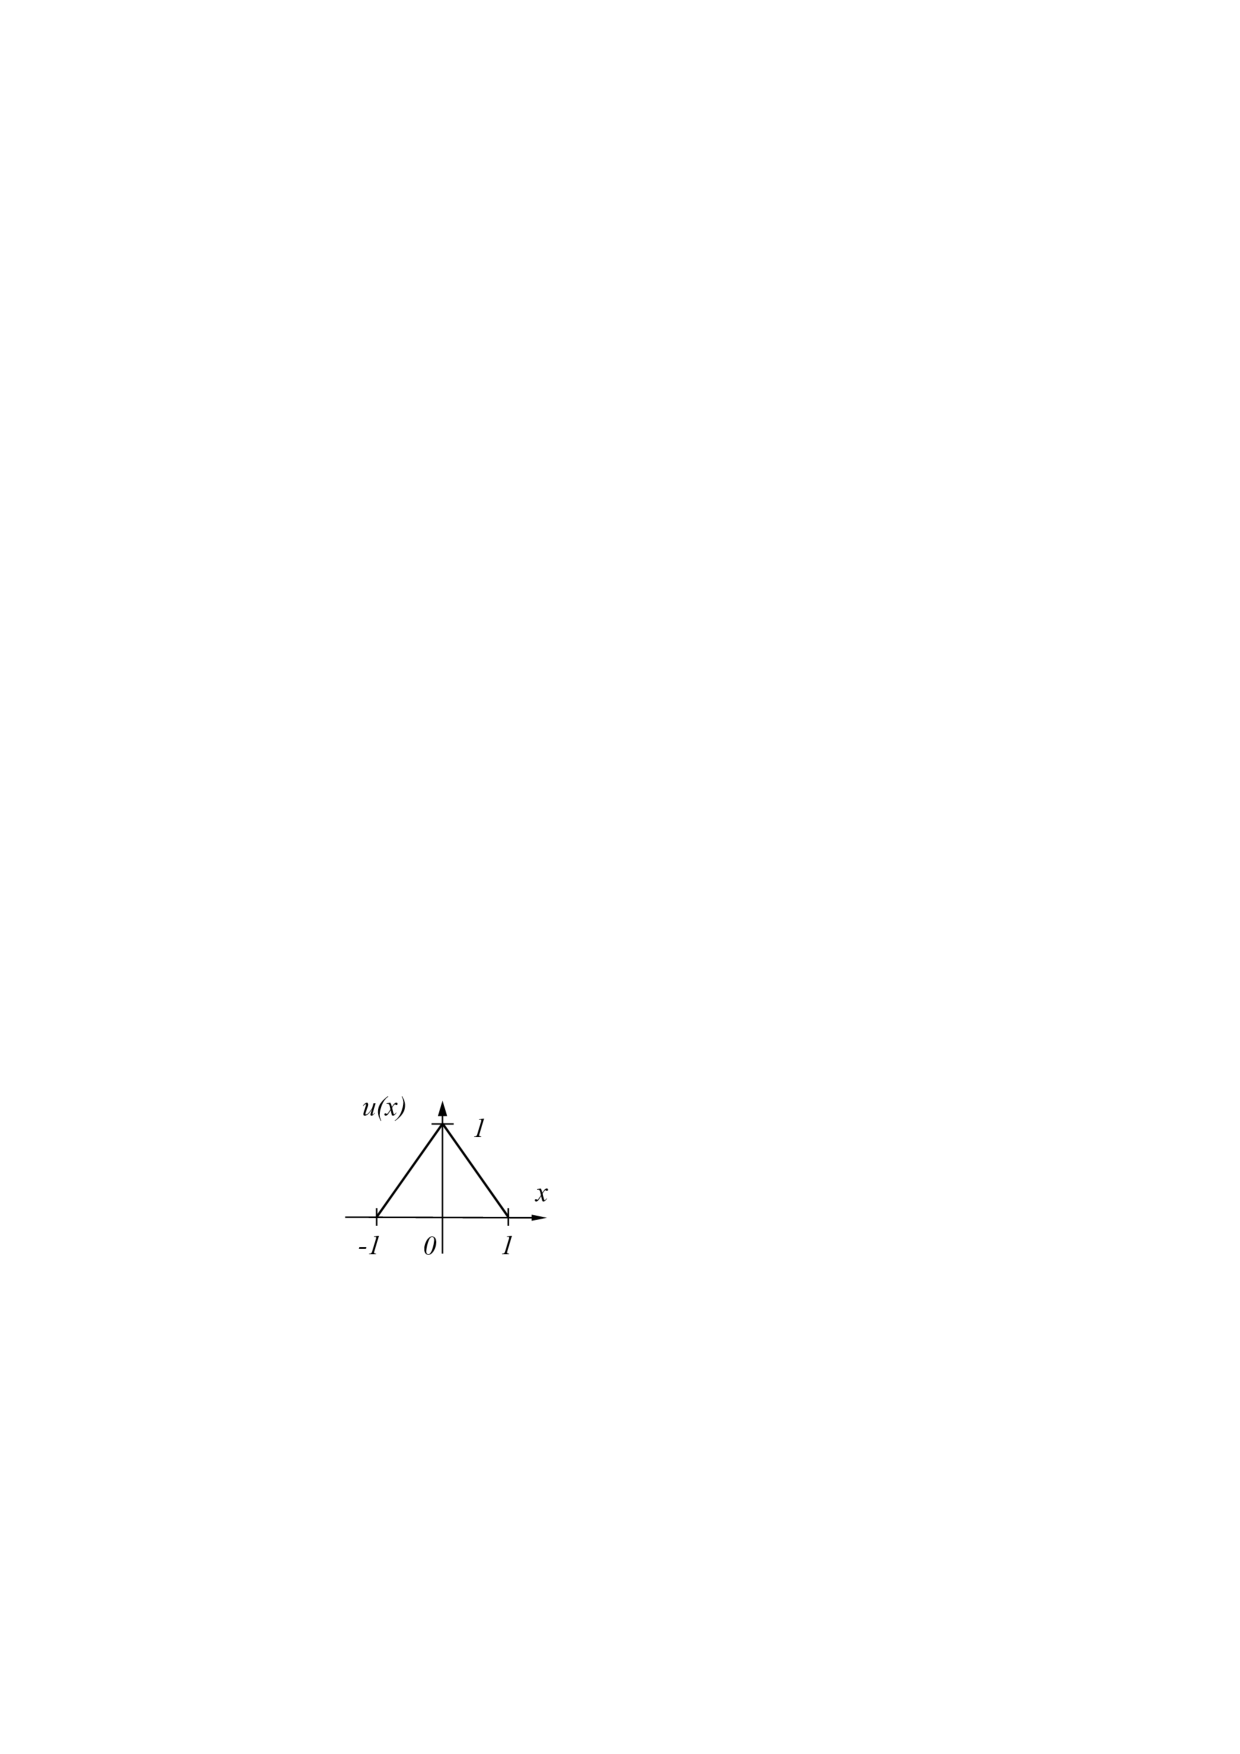
\includegraphics[width=0.5\linewidth]{img/hut}
		\caption[Hutfunktion]{Hutfunktion}
		\label{fig:hut}
	\end{figure}


	
	Setzen wir dies nun in die Herleitung der schwachen Formulierung \ref{weak-form} ein, erhalten wir mit etwas umformen und unter Verwendung der verallgemeinerten Ableitung aus Formel \ref{distribution-differential}. Da sich unser Intervall zeitlich nicht �ndert, darf die Zeit-Ableitung vor das Integral gezogen werden (???).
	\begin{equation}
	\sum_{i = 0}^{N} u_i   \int_{a}^{b} p_i'(x) v'(x) dx - 
	\mu_0 \epsilon_0 \frac{\partial ^2 }{\partial t^2} \sum_{i = 0}^{N} u_i \int_{a}^{b}p_i(x)v(x) dx = 0
	\label{weak-form2}
	\end{equation}
	Hier gelten noch $u_1,u_2,...u_N$, also $N$ Unbekannte Koeffizienten, zu finden. F�r $N$ unbekannte Koeffizienten werden bekanntlich $N$ unabh�ngige Gleichungen ben�tigt. Ein Weg diese zu erhalten ist �ber die Ansatzfunktion $v(x)$. F�r diese Ansatzfunktion wird ebenfalls eine �hnliche Zerlegung wie f�r $p(x)$ festgelegt, sollte es sogar die selbe sein, handelt es sich um die \textit{Galerkin Methode}. Man setzt also
	\begin{equation}
	v(x) = p(x) = \sum_{j = 0}^{N} p_j(x)
	\end{equation}
	und setzt dies dann in die Gleichung (\ref{weak-form2}) ein.
	\begin{equation}
	\sum_{i = 0}^{N} u_i \sum_{j = 0}^{N}\int_{a}^{b} p_i' p_j' dx 
	+ 
	\sqrt{\mu \epsilon} \frac{\partial}{\partial t} u_i \sum_{j = 0}^{N} p_i(B) p_j
	= 
	\mu \epsilon \sum_{i = 0}^{N} \frac{\partial ^2 }{\partial t^2} u_i 
	\sum_{j = 0}^{N} \int_{a}^{b} p_i p_j dx
	\end{equation}
	
	Da wir Hutfunktionen verwenden k�nnen, welche durch die Dreiecksfunktion $p_i = tri(\frac{x + ih}{h})$ beschrieben werden, k�nnen die Integrale gel�st werden:
	
	\begin{equation}
	\int_{a}^{b} p_ip_j dx = \begin{cases}
	\frac{4}{6}h, ~~ j=i \\
	\frac{1}{6}h,~~ j=\{i-1,i+1\}\\
	0\, ~~\text{sonst}
	\end{cases}
	\end{equation}
	und f�r $p'_i p'_j$ gilt
	\begin{equation}
	\int_{a}^{b} p_i' p_j' dx = \begin{cases}
	\frac{2}{h}, ~~ j=i \\
	-\frac{1}{h},~~ j=\{i-1,i+1\}\\
	0\, ~~\text{sonst}
	\end{cases}
	\end{equation}
	
	\begin{figure}
		\centering
		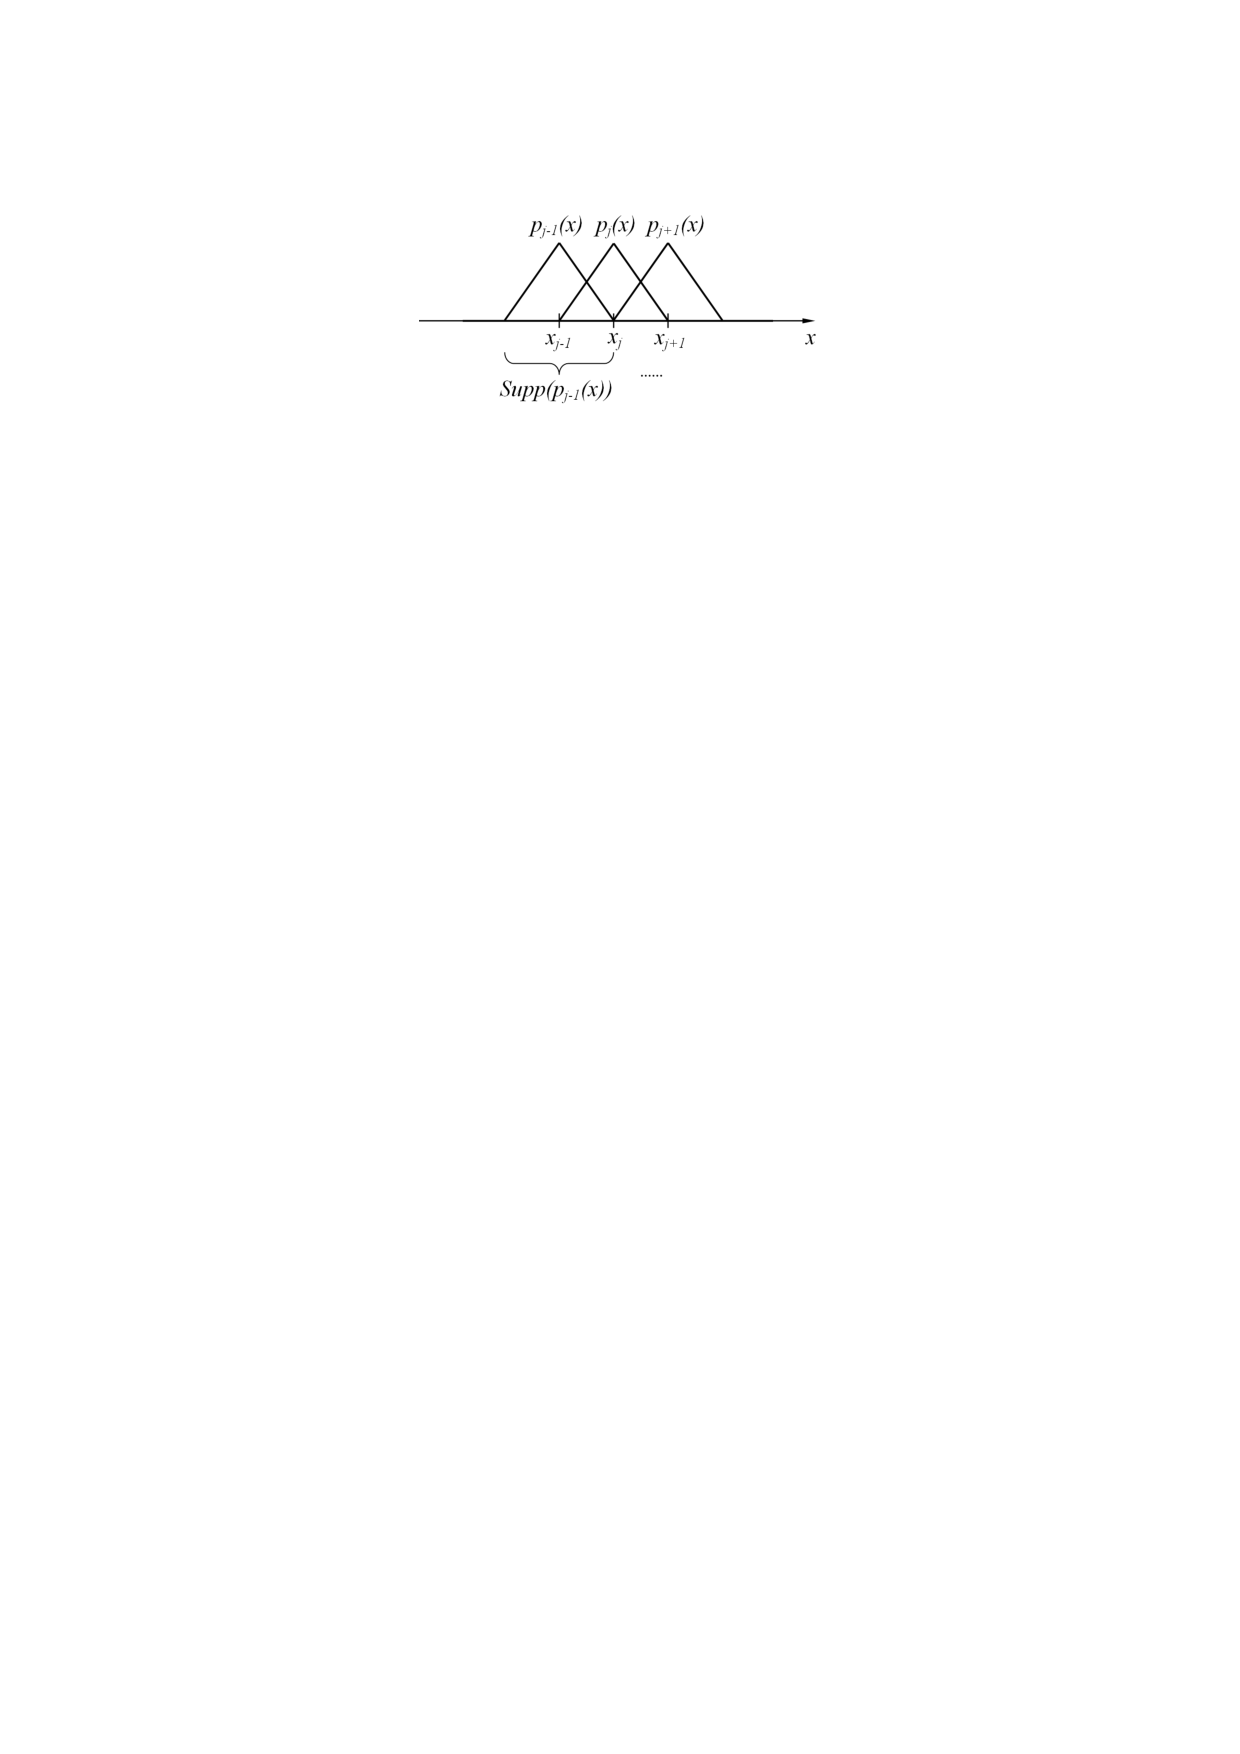
\includegraphics[width=0.7\linewidth]{img/hutfunktionen}
		\caption{�berlagerte Hutfunktionen}
		\label{fig:hutfunktionen}
	\end{figure}
	
	Damit kann das Gleichungssystem in der Form
	
	\begin{equation}
	\mathbf{S}_h \mathbf{u}_h + \mathbf{C}_h \frac{\partial}{\partial t} \mathbf{u}_h + \mathbf{M}_h \frac{\partial ^2}{\partial t^2} \mathbf{u}_h = \mathbf{0}
	\end{equation}
	
	folgenderma�en angeschrieben werden:
	
	\begin{equation}
	\begin{split}
	\frac{1}{h}   
	\begin{bmatrix}
	2 & -1 & 0 & \cdots & 0 \\ 
	-1 & 2 & -1 & \cdots & 0 \\ 
	0 & -1 & 2 & \ddots & \vdots \\ 
	\vdots & \vdots & \ddots & \ddots & -1 \\ 
	0 & 0 & \cdots & -1 & 2
	\end{bmatrix} 
	\begin{bmatrix}
	u_1 \\ 
	u_2 \\ 
	\vdots \\ 
	u_N
	\end{bmatrix}  +
	\sqrt{\mu_0 \epsilon_0} 
	\frac{\partial}{\partial t} 
	\begin{bmatrix}
	0 \\ 
	0 \\ 
	\vdots \\ 
	u_N
	\end{bmatrix}
	+ \\ +
	\mu_0 \epsilon_0 \frac{h}{6}
	\begin{bmatrix}
	4 & 1 & 0 & \cdots & 0 \\ 
	1 & 4 & 1 & \cdots & 0 \\ 
	0 & 1 & 4 & \ddots & \vdots \\ 
	\vdots & \vdots & \ddots & \ddots & 1 \\ 
	0 & 0 & \cdots & 1 & 4
	\end{bmatrix} 
	\frac{\partial ^2}{\partial t^2} 
	\begin{bmatrix}
	u_1 \\ 
	u_2 \\ 
	\vdots \\ 
	u_N
	\end{bmatrix} = 
	\begin{bmatrix}
	0 \\ 
	0 \\ 
	\vdots \\ 
	0
	\end{bmatrix}
	\end{split}
	\end{equation}
	
	\subsection{Newmark Zeitschrittverfahren}
	
	Hier werden die partiellen Zeitableitung durch die Variablen $u, v, a$ dargestellt.
	\[
	u = u(t_j) , \quad 
	\frac{\partial u}{\partial t} \approx v(t_j) , \quad
	\frac{\partial^2 u}{\partial t^2} \approx a (t_j)
	\]
	Diese sind eine Anlehnung an die Mechanik, wo die erste Ableitung des Weges nach der Zeit die Geschwindigkeit $v$, und die zweite Ableitung nach der Zeit die Beschleunigung $a$ bezeichnet.
	Das Newmark-Verfahren beruht auf einer Taylor-Entwicklung f�r $u$ und $v$, wobei
zweite Ableitungen durch Beschleunigungen zum Zeitpunkt $t_j$ und $t_{j+1}$ approximiert werden. F�r den Zeitpunkt $t_{j+1} = tj + \Delta t$ ergibt sich das Gleichungssystem
	
	\begin{equation}
	\mathbf{Su}_{j+1} + 	\mathbf{Cv}_{j+1} +	\mathbf{Ma}_{j+1} = 	\mathbf{f}_{j+1}
	\label{eq:newmark}
	\end{equation}
	
	\begin{align}
		v_{j+1} &= v_j + \Delta t  [(\frac{1}{2}-\gamma)a_j + \gamma a_{j+1}] \\
		u_{j+1} &= u_j + \Delta t v_j + \frac{(\Delta t)^2}{2} [(\frac{1}{2}-\beta)a_j + \beta a_{j+1}]
	\end{align}
	
	mit $\beta = \frac{1}{4}$ und $\gamma = \frac{1}{2}$.
	
	Die Gleichung \ref{eq:newmark} kann auf einen der drei Parameter umgeformt werden und es ergibt sich
	\begin{equation}
	(\mathbf{S} + \gamma \Delta t	\mathbf{C} +	\mathbf{M})a_{j+1} = 	\mathbf{\tilde f}_{j+1}
	\label{eq:newmark-final}
	\end{equation}
	wobei die Gr��en $u_j$, $v_j$ und $a_j$ in den Vektor $\mathbf{\tilde f}_{j+1}$ sind. Herleitung siehe Skriptum.
	
	
	\subsection{Implementierung in Matlab}
	\lstinputlisting[language=matlab,style=myMatlabStyle,caption={Implementierung der FEM f�r ein eindimensionales L�sen der Wellengleichung}]{../Matlab/FEM.m}	
	
	\pagebreak
	\subsection{Ergebnis}
	
	Die Methode der finiten Elemente in Kombination mit dem Newmark'schen Zeitschrittverfahren bringt sehr brauchbare Ergebnisse hervor. Jedoch neigt das Verfahren, trotz einhalten der Stabilit�tsbedingung
	\begin{equation}
		\Delta t < \frac{\Delta x^2}{v}
	\end{equation}
	 zur Instabilit�t.

	
	\begin{figure}[!h]
		\centering
		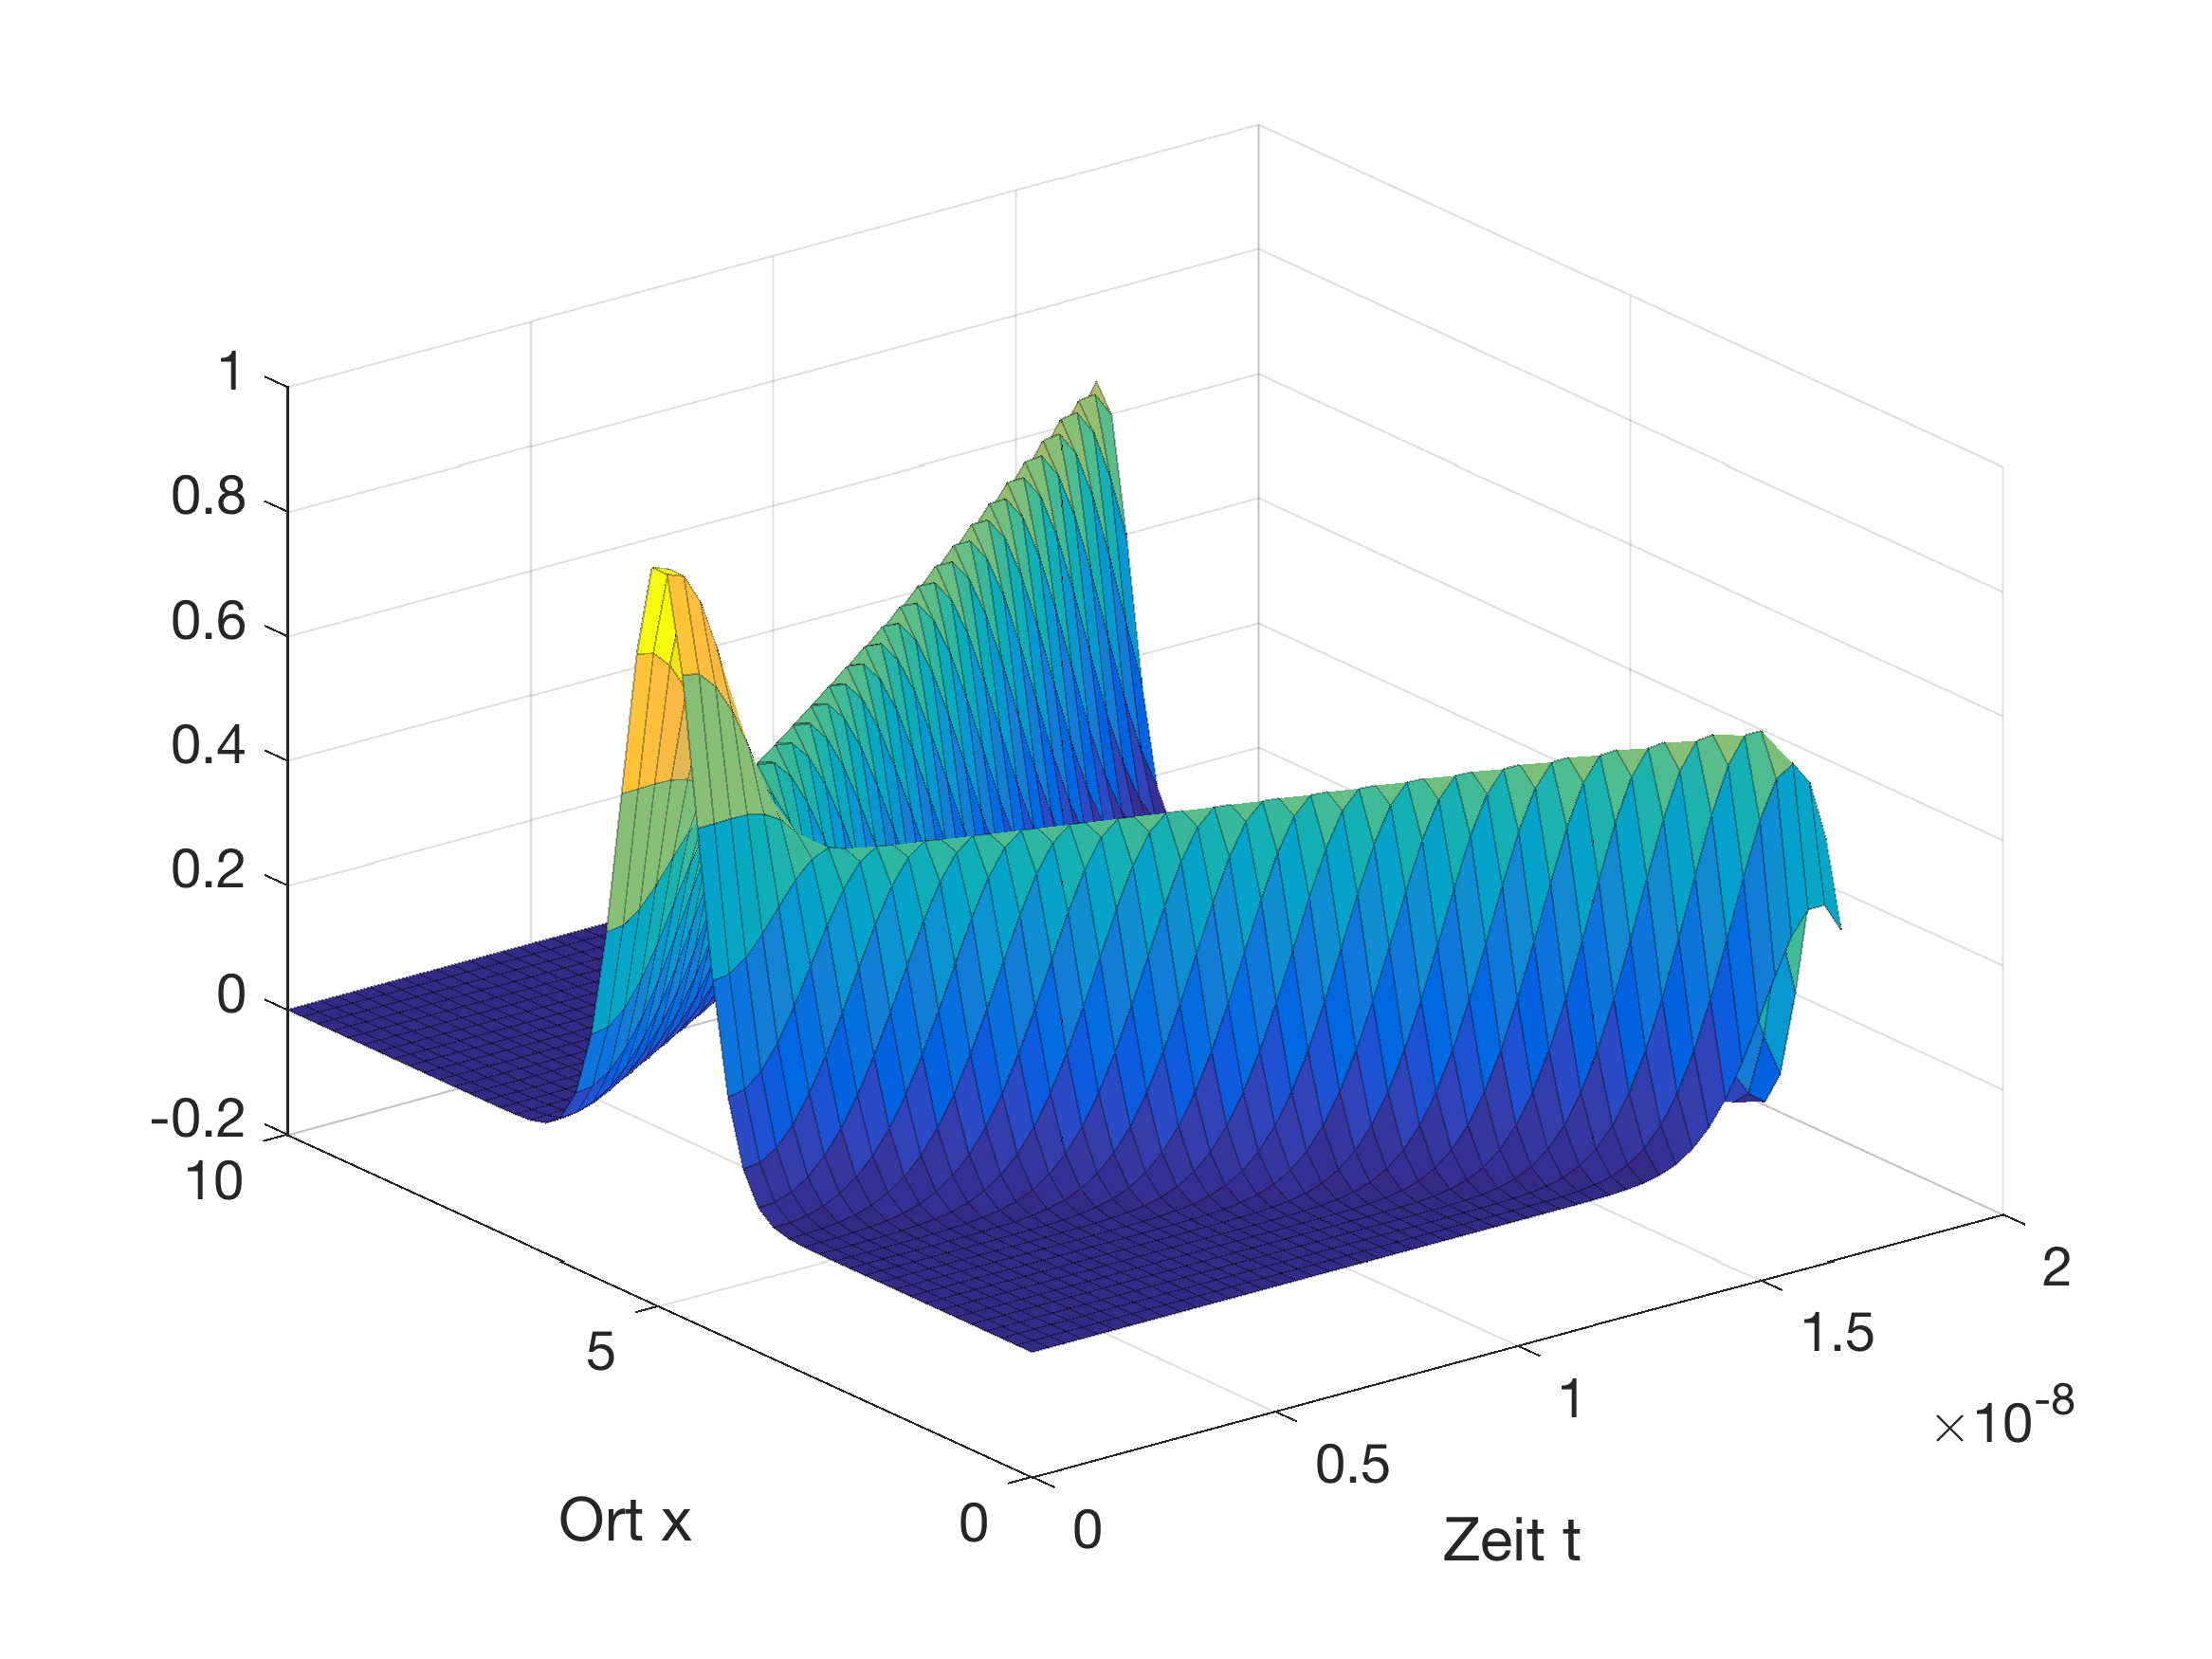
\includegraphics[width=\linewidth]{../Matlab/wave}
		\caption{Ergebnisse der FEM mit dem Newmark-Zeitschrittverfahren}
		\label{fig:wave}
	\end{figure}
	